\begin{figure}[H]
	\centering
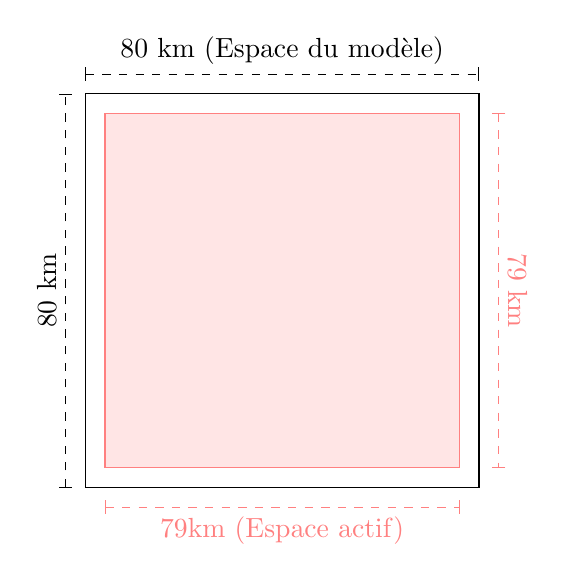
\begin{tikzpicture}[scale=.5]
\draw[] (0,0) -- (0,10) -- (10,10) -- (10,0) -- cycle;
\draw[|-|, very thin, dashed] (0, 10.5) -- node[above] {80 km (Espace du modèle)} (10, 10.5);
\draw[|-|, very thin, dashed] (-0.5, 0) -- node[above, rotate=90] {80 km} (-0.5, 10);

\draw[color=red!50, fill = red!10] (0.5, 0.5) -- (0.5, 9.5) -- (9.5, 9.5) -- (9.5, 0.5) -- cycle;
\draw[|-|, very thin, dashed, red!50] (10.50, 9.50) -- node[above, red!50, rotate=-90] {79 km} (10.5, 0.5);
\draw[|-|, very thin, dashed, red!50] (0.5, -0.5) -- node[below, red!50] {79km (Espace actif)} (9.5, -0.5);
\end{tikzpicture}
\caption{L'espace support de SimFeodal, un monde théorique.\\
N.B : Dans le schéma, pour une question de lisibilité, les dimensions de l'espace réduit ne sont pas proportionnelles à celles de l'espace d'ensemble.}
\label{fig:espace-simfeodal}
\end{figure}